\chapter{Estudo de Caso: projeto Mezuro}
\label{cap-estudo-caso}

O trabalho de pesquisa desenvolvido durante o capítulo \ref{cap-usabilidade}, onde se levantou técnicas de usabilidade ágeis que poderiam ser aplicadas na comunidade de software livre conforme seção \ref{técnicas-usabilidade-ageis} e depois a seleção de uma dessas técnicas a fim de realizar sua descrição e detalhamento na seção \ref{usabilidade-sl} tinha como objetivo definir a forma que seria integrado a usabilidade em uma equipe de desenvolvimento em um contexto de software livre. Detalhar essa forma de trabalho se faz necessário, pois esses conceitos e métodos serão apresentados e aplicados em uma ferramenta real que será utilizada como estudo de caso.

%
YIN (\citeyear{yin2009}) diz que "o estudo de caso é uma inquirição empírica que investiga um fenômeno contemporâneo dentro de um contexto da vida real, quando a fronteira entre o fenômeno e o contexto não é claramente evidente e onde múltiplas fontes de evidência são utilizadas".
Validar a pesquisa através de sua aplicação trás vantagens como:
\begin{itemize}
\item Produção de artefatos descritivos suficientemente rico para permitir reinterpretações subsequentes.
\item Relacionamento da teoria com a prática
\item Melhor percepção através de exemplos específicos, acontecimentos ou experiências
\end{itemize}

%
Segundo YIN (\citeyear{yin2009}), para um estudo de caso deve se definir:
\begin{itemize}
\item Uma visão geral do projeto do estudo de caso
\item Os procedimentos que serão aplicados, abordados
\item As questões do estudo de caso que o investigador deve ter em mente, os locais, as fontes de informação, os formulários para o registro dos dados e as potenciais fontes de informação para cada questão
\item Um guia para o relatório do Estudo do Caso
\end{itemize}

%
A definição dessa estrutura se dá de forma automática devido ao modelo adotado de abordagem da usabilidade dentro do projeto facilitando a aplicação do método.

A ferramenta definida para o estudo de caso foi o software livre Mezuro, uma plataforma de monitoramento de código-fonte. A escolha desta ferramenta se deve ao fato que, ao ser concebida, um trabalho similar foi realizado pela pesquisadora Ana Paula Oliveira dos Santos, porém a ferramenta se tratava de um plugin de outra plataforma e tornou-se necessário uma migração para uma ferramenta standalone. Com essa troca muito foram as mudanças e os aspectos de usabilidade passaram a necessitar de um novo planejamento.Outro fator importante foi a facilidade de estar inserido junto a equipe de desenvolvimento, ficando assim mais próximo do projeto.

\section{Mezuro}
\label{mezuro}

A plataforma Mezuro foi concebida com o intuito de comparar projetos e métricas técnicas,
ensinar como usar métricas através de configurações, analisar o código, evitar dívidas técnicas e divulgar o uso de métricas de código.

O contexto da plataforma é descrito de forma resumida pelos seu desenvolvedores da seguinte forma:
\begin{description}
\item[Para] desenvolvedores de software
\item[que] precisam de um melhor entendimento sobre o seu próprio código
\item[o] Mezuro
\item[é uma] rede social de nicho
\item[que] fornece interpretação métrica colaborativa.
\item[Ao contrário] CodeClimate
\item[nosso projeto] atende várias linguagens, tem configurações abertas para avaliações de código e tudo isso de graça
\end{description}

De forma técnica o Mezuro é uma plataforma para analisar e compreender as métricas, bem como, aplicar os conceitos de código limpo, medição de software e atratividade do software livre. Ele é um software livre sob licença AGPL~\footnote{GNU Affero General Public License (AGPL): \url{gnu.org/licenses/agpl.html}}. Mezuro usa Kalibro Metrics , que é um serviço web que pode se conectar a diferentes tipos de repositórios de código-fonte , baixar projetos de software e executar muitos coletor métrica integrada e ferramentas de calculadora automaticamente. Kalibro é licenciado LGPL~\footnote{GNU Lesser General Public License (LGPL):\url{gnu.org/licenses/lgpl.html}}~\cite{mezuro2012}.
É uma aplicação Web para que os líderes e desenvolvedores de projetos de software livre possam monitorar características de código-fonte, através de métricas de acoplamento, coesão, tamanho, encapsulamento, entre outras. Isso proporciona um acompanhamento do quanto o software está crescendo e se tornando mais complexo em relação a ele mesmo e à média dos projetos avaliados pelo Mezuro~\cite{santos2012}
.

A plataforma Mezuro foi desenvolvida no contexto do projeto QualiPSo (\textit{Trust and Quality in Open Source Systems}).
O projeto integrado Qualipso (Quality Plataform for Open Source) busca definir e implementar tecnologias, procedimentos, leis e políticas com o objetivo de potencializar as práticas de desenvolvimento de software livre, tornando-as confiáveis, reconhecidas e estabelecidas na indústria.
Para viabilizar o projeto e a sustentação do software livre como uma solução confiável para a indústria, criou-se um consórcio formado por colaboradores de diferentes origens: França, Itália, Brasil, Espanha, China, Alemanha e Escócia~\cite{qualipso2013}
.

Para o desenvolvimento do Mezuro realizou-se um estudo de plataformas correlatas a fim de melhor situar as resoluções já existentes~\cite{meirelles2013}%Paulo Meirelles
. As ferramentas estudadas foram:

\begin{description}
\item[FLOSSMetrics (Free /Libre Open Source Software Metrics)]
é um projeto que utiliza metodologias e ferramentas existentes para fornecer um grande banco de dados com informações sobre o desenvolvimento de software livre
\item[Ohloh]
é uma plataforma que oferece um conjunto de serviços web e um sistema web para comunidade de software livre, que visa prover uma visão geral de evolução dos projetos de software livre em desenvolvimento
\item[Qualloss (Quality in Open Source Software)]
é uma metodologia para automatizar a medição da qualidade de projetos de software livre, usando ferramentas para analisar o código-fonte e as informações dos repositórios dos projetos
\item[SQO-OSS (Software Quality Assessment of Open Source Software)]
fornece um conjunto de ferramentas para análise e avaliação comparativa de projetos de software livre
\item[QSOS]
é uma metodologia baseada em quatro etapas: definição de referência utilizada; avaliação de software; qualificação dos usuários em contexto específico; seleção e comparação de software
\item[FOSSology]
(Advancing open source analysis and development) é um projeto que fornece um banco de dados gratuito com informações sobre licenças de software livre
\item[HackyStat]
é um ambiente para visualização, análise e interpretação do processo de desenvolvimento de software e dados do produto de software
\end{description}

\subsection{Mezuro Plugin}
\label{mezuro-plugin}
A primeira versão da ferramenta foi desenvolvida sendo uma instância da plataforma de rede social Noosfero 6 com o plugin Mezuro ativado. Noosfero é um software livre (plataforma web) para redes sociais que possui as funcionalidades de Blog, e-Portfolios, RSS, discussão temática e agenda de eventos em um único sistema. Ele foi desenvolvido em linguagem de programação Ruby usando o framework Rails. Ruby on Rails é baseado em arquitetura Model View Controller (MVC). Plugins Rails (como Mezuro plugin) é uma extensão do quadro principal, assim, a arquitetura Mezuro também foi baseada em MVC, seguindo Rails e a arquitetura do Noosfero~\cite{mezuro2012}.

\begin{figure}[H]
  \begin{center}
    \includegraphics[width=0.5\textwidth]{figuras/arquitetura.eps}
    \caption{Interação Mezuro e Kalibro Metrics}
    \label{fig:arquitetura}
  \end{center}
\end{figure}

A utilização de plugins permitem que os desenvolvedores possam resolver 
vários problemas sem interagir com a base de código inteira. O Mezuro foi 
o primeiro plugin do Noosfero, sua estrutura foi construída sobre um 
paradigma baseado em eventos.O Noosfero dispara um evento em um 
determinado ponto e todos os plugins interessados nesse evento são 
capazes de agir. O Mezuro se comunica com o Kalibro Métricas Web Service, 
como mostrado na Figura \ref{fig:arquitetura}, via solicitações SOAP, que 
prove o acesso aos seguintes end-points do Kalibro Services: Kalibro,
Project, ProjectResult, ModuleResult, BaseTool, Configuration, e 
MetricConfiguration. Do ponto de vista conceitual, cada end-point Kalibro 
é um serviço do Mezuro que funciona como um orquestrador dos sete 
serviços, uma vez que cada um trabalha de forma independente e tem um 
conjunto diferente de funcionalidades. O Mezuro chama cada end-point 
(serviço ) de acordo com suas ações (pedidos) para o Kalibro. Em suma, o 
desempenho e a escalabilidade do Mezuro dependem desta "orquestração".
~\cite{mezuro2012}

\subsection{Mezuro Standalone}
\label{mezuro-standalone}

O mezuro standalone surgiu da necessidade de portar o mezuro plugin para uma plataforma independente do Noosfero. Isso ocorreu devido à limitações ocasionadas pelo Noosfero. Uma dessas limitacoes deve-se ao fato de seu desenvolvimento ser baseado em uma versão do antiga do rails com pouco suporte pela comunidade e limitado as funções dessa versão.
O mezuro standalone é baseado no framework rails 4.0, utiliza-se BootStrap para o desenvolvimento de interface (front-end) e permanece com o protocolo de comunicação SOAP entre o mezuro e o kalibro conforme descrito na seção anterior, porém estuda-se uma possível mudança para JSON.
O mezuro standalone é um novo ciclo de desenvolvimento da plataforma Mezuro. Este encontra-se em fase de criação o que permite aplicar a usabilidade dentro do ciclo de vida do projeto juntamente com a equipe de desenvolvimento.

Seguindo as técnicas de usabilidade adotas, descrita na seção \ref{usabilidade-sl}, as tarefas de usabilidade a serem realizadas no projeto Mezuro serão:
\begin{itemize}
\item Coletar requisitos de tarefas e necessidades dos usuários
\item Criar protótipos de tela
\item Testar protótipos com avaliações heurísticas
\item Testar a usabilidade de protótipos com usuários locais e remotos (manipulação de variáveis independentes)
\item Coletar métricas (variáveis dependentes)
\item Apresentar resultados das análises dos testes (tracking)
\item Definição de histórias de usabilidade baseadas nos requisitos fornecidos pelos clientes e no resultado dos testes de us
\item Implementação das histórias definidas
\end{itemize}

Estes artefatos gerados levam em consideração os seguinte aspectos de usabilidade~\cite{ergolist2013}:

\begin{description}
\item[Presteza]
verifica se o sistema informa e conduz o usuário durante a interação.
\item[Agrupamento por localização]
Verifica se a distribuição espacial dos itens traduz as relações entre as informações.
\item[Agrupamento por formato]
Verifica os formatos dos itens como meio de transmitir associações e diferenças.
\item[Feedback]
Avalia a qualidade do feedback imediato às ações do usuário.
\item[Legibilidade]
Verifica a legibilidade das informações apresentadas nas telas do sistema.
\item[Concisão]
Verifica o tamanho dos códigos e termos apresentados e introduzidos no sistema.
\item[Ações Mínimas]
Verifica a extensão dos diálogos estabelecidos para a realização dos objetivos do usuário.
\item[Densidade Informacional]
Avalia a densidade informacional das telas apresentadas pelo sistema.
\item[Ações Explícitas]
Verifica se é o usuário quem comanda explicitamente as ações do sistema.
\item[Controle do Usuário]
Avalia as possibilidades do usuário controlar o encadeamento e a realização das ações.
\item[Flexibilidade]
Verifica se o sistema permite personalizar as apresentações e os diálogos.
\item[Experiência do Usuário]
Avalia se usuários com diferentes níveis de experiência têm iguais possibilidades de obter sucesso em seus objetivos.
\item[Proteção contra erros]
Verifica se o sistema oferece as oportunidades para o usuário prevenir eventuais erros.
\item[Mensagens de erro]
Avalia a qualidade das mensagens de erro enviadas aos usuários em dificuldades.
\item[Correção de erros]
Verifica as facilidades oferecidas para que o usuário possa corrigir os erros cometidos.
\item[Consistência]
Avalia se é mantida uma coerência no projeto de códigos, telas e diálogos com o usuário.
\item[Significados]
Avalia se os códigos e denominações são claros e significativos para os usuários do sistema.
\item[Compatibilidade]
Verifica a compatibilidade do sistema com as expectativas e necessidades do usuário em sua tarefa.
\end{description}

Desses artefatos um deles são os protótipos de telas que visam instruir a equipe de desenvolvimento. Nesses protótipos são inserido as considerações da equipe, requisitos do projeto, experiência do responsável pela usabilidade e alguns dos aspectos apresentados. Os protótipos desenvolvidos e apresentados para a equipe de uma primeira feature foram:
 
\begin{figure}[H]
  \begin{center}
    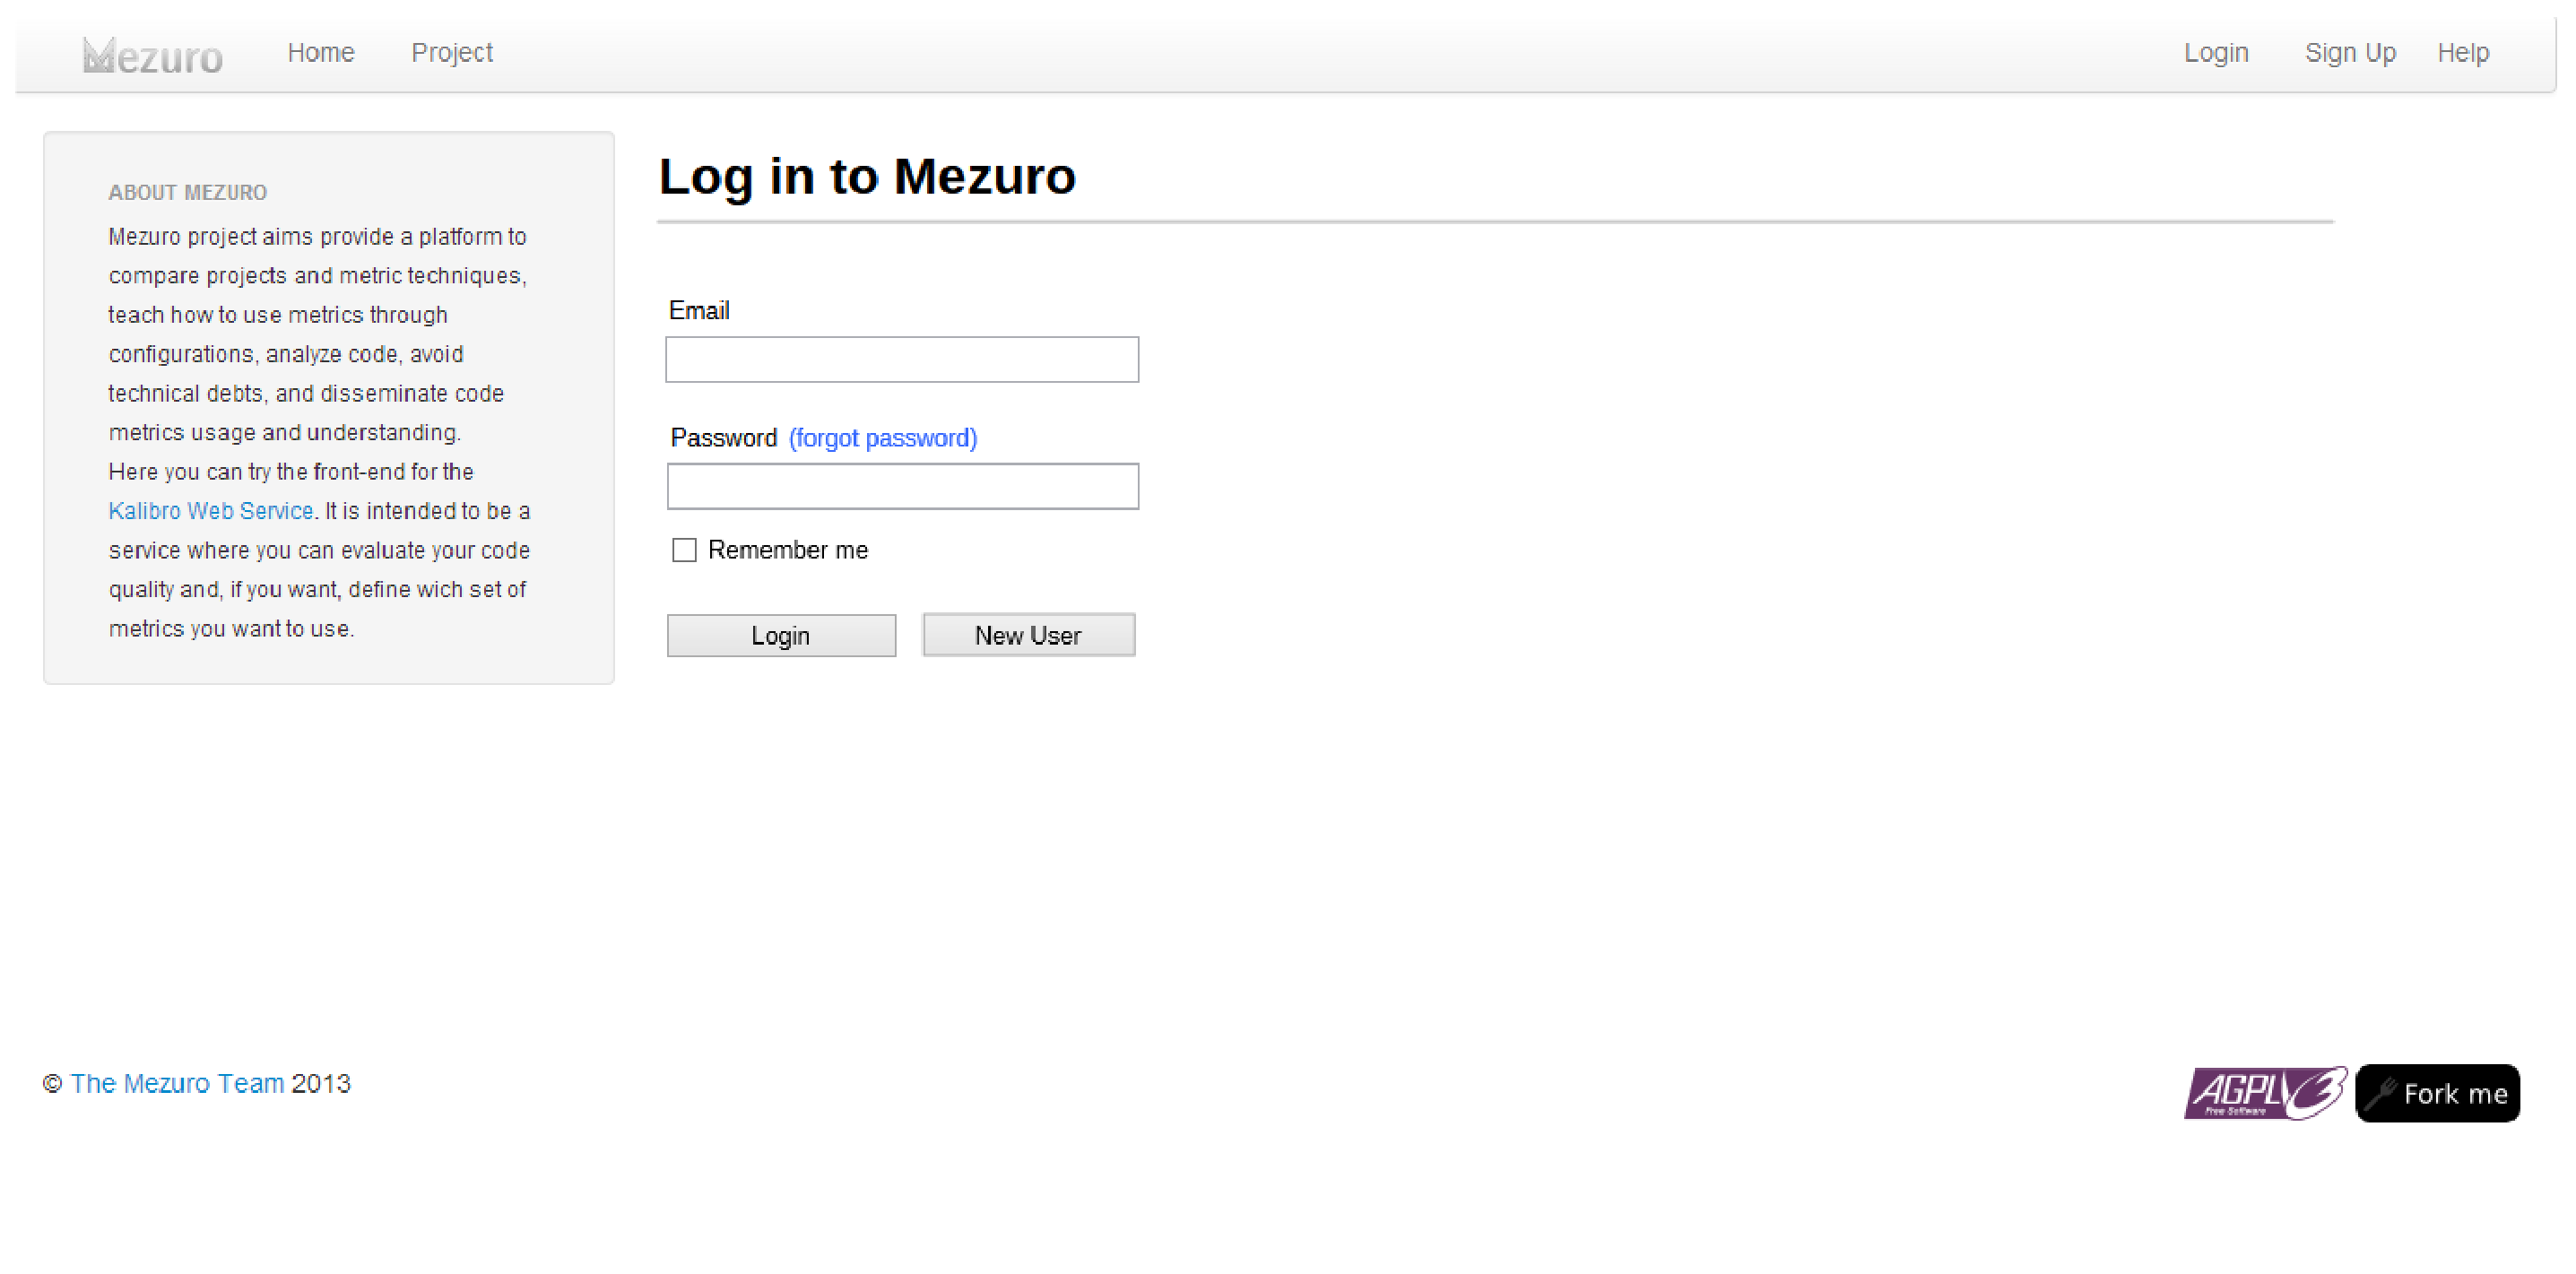
\includegraphics[width=1\textwidth]{figuras/Login.eps}
    \caption{Protótipo de tela: Login}
    \label{fig:pLogin}
  \end{center}
\end{figure}

\begin{figure}[H]
  \begin{center}
    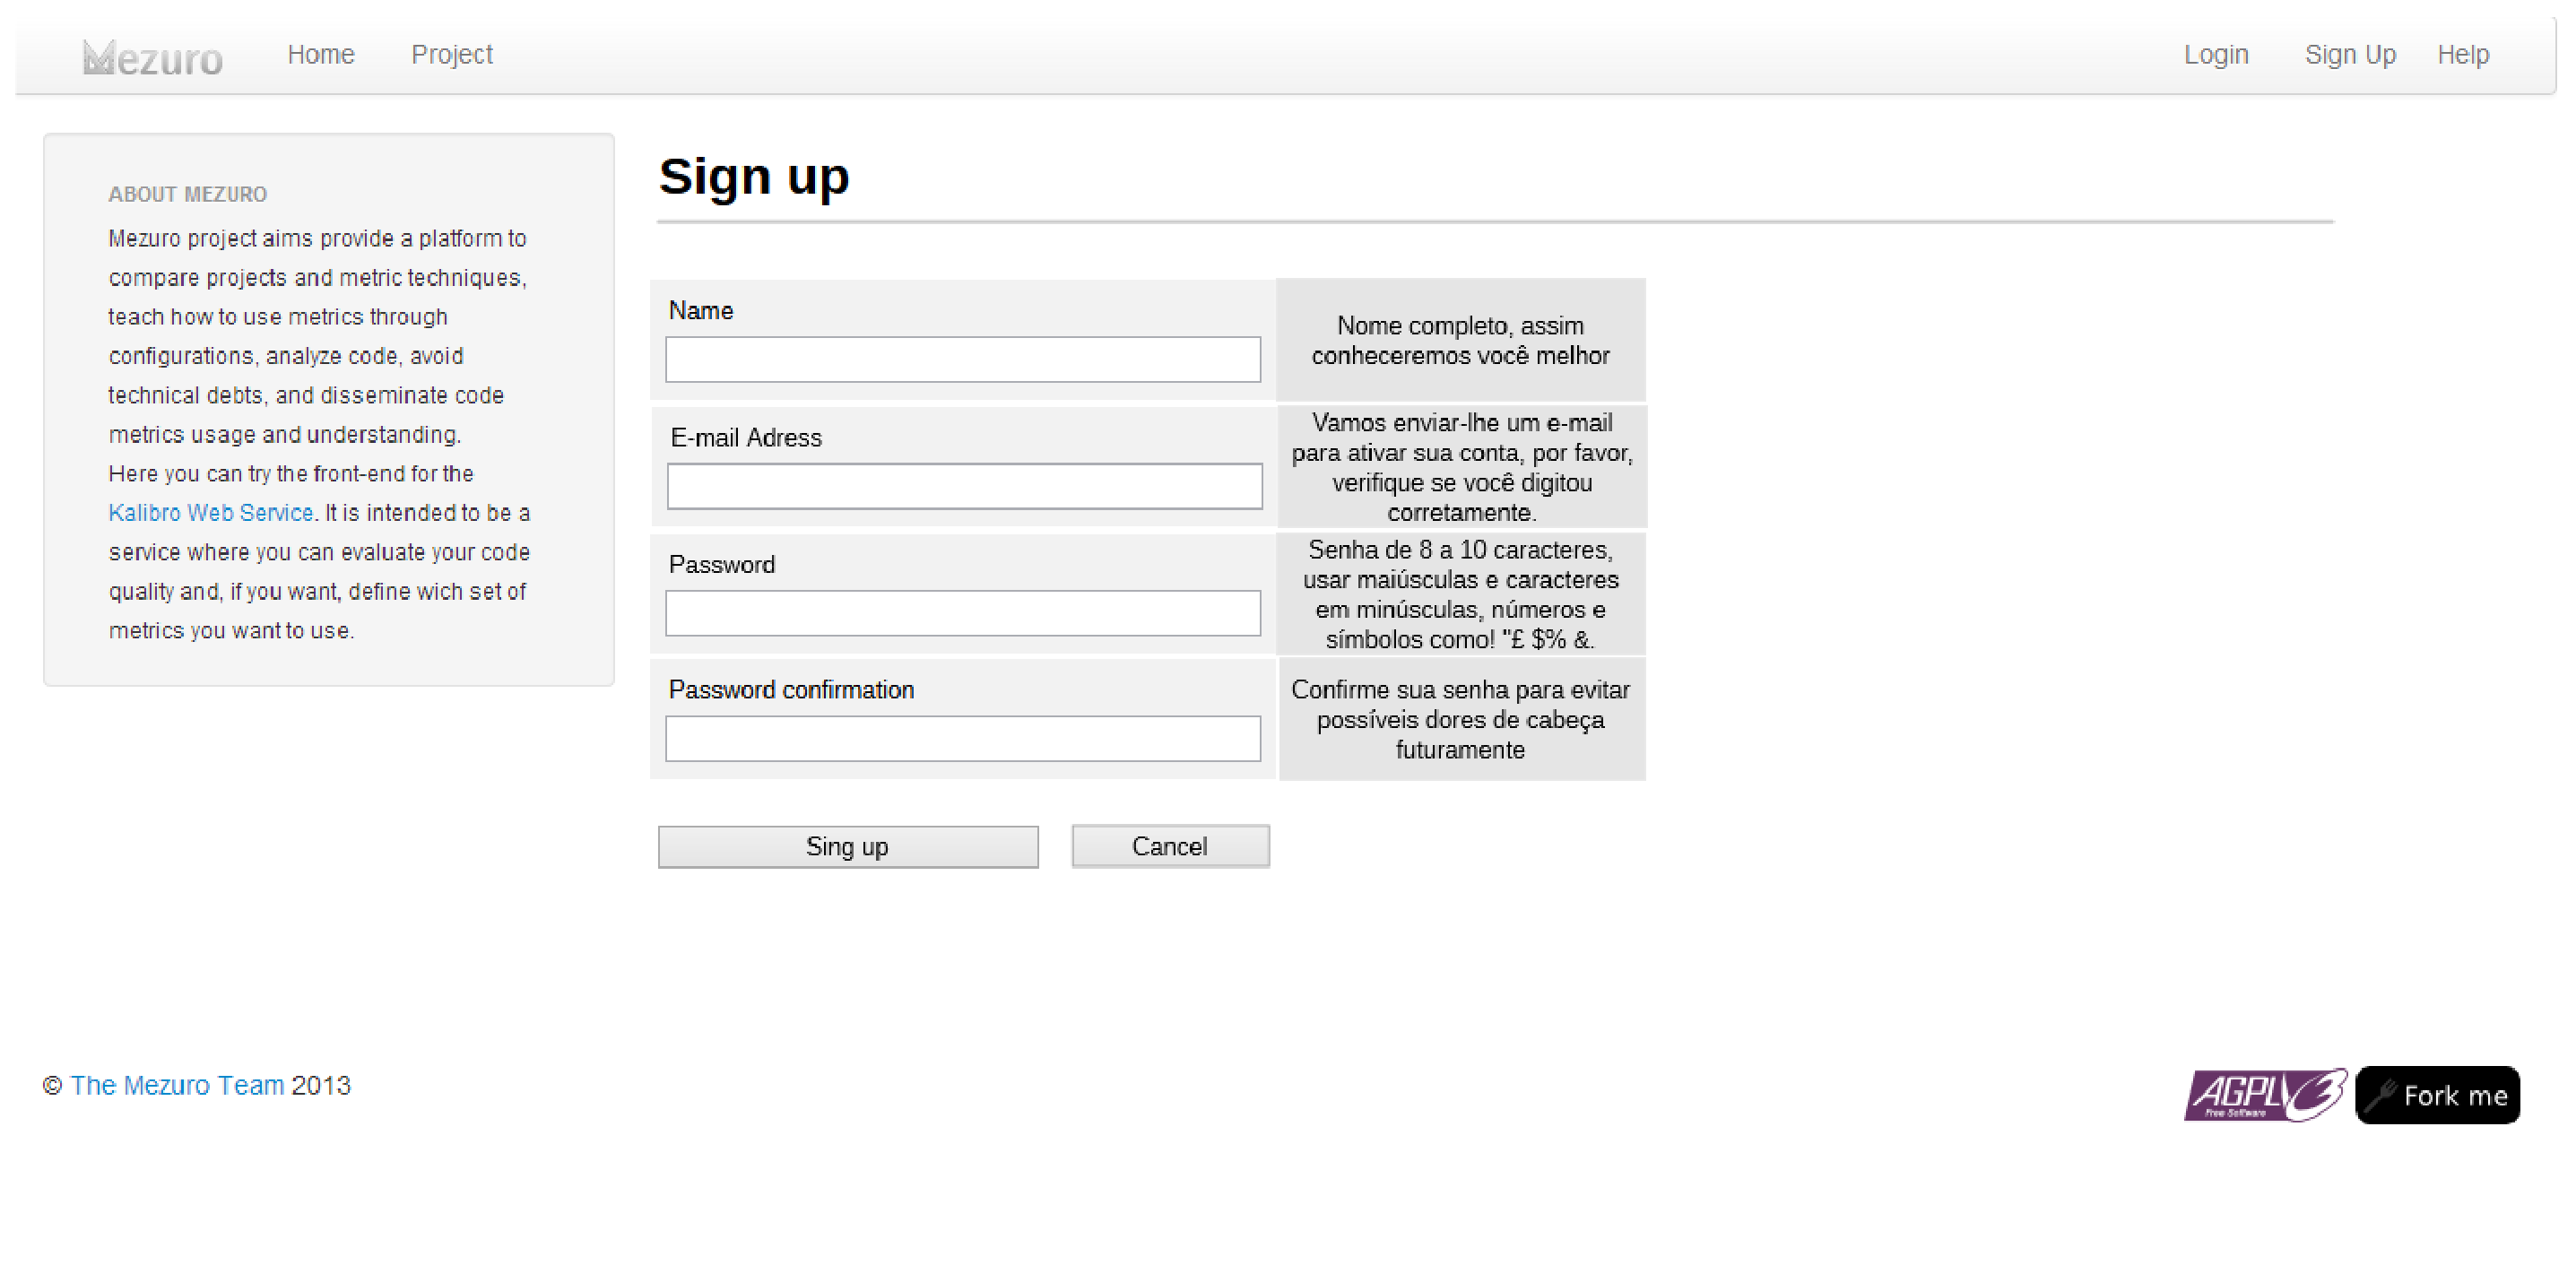
\includegraphics[width=1\textwidth]{figuras/Signup.eps}
    \caption{Protótipo de tela: Signup}
    \label{fig:pSignup}
  \end{center}
\end{figure}

\begin{figure}[H]
  \begin{center}
    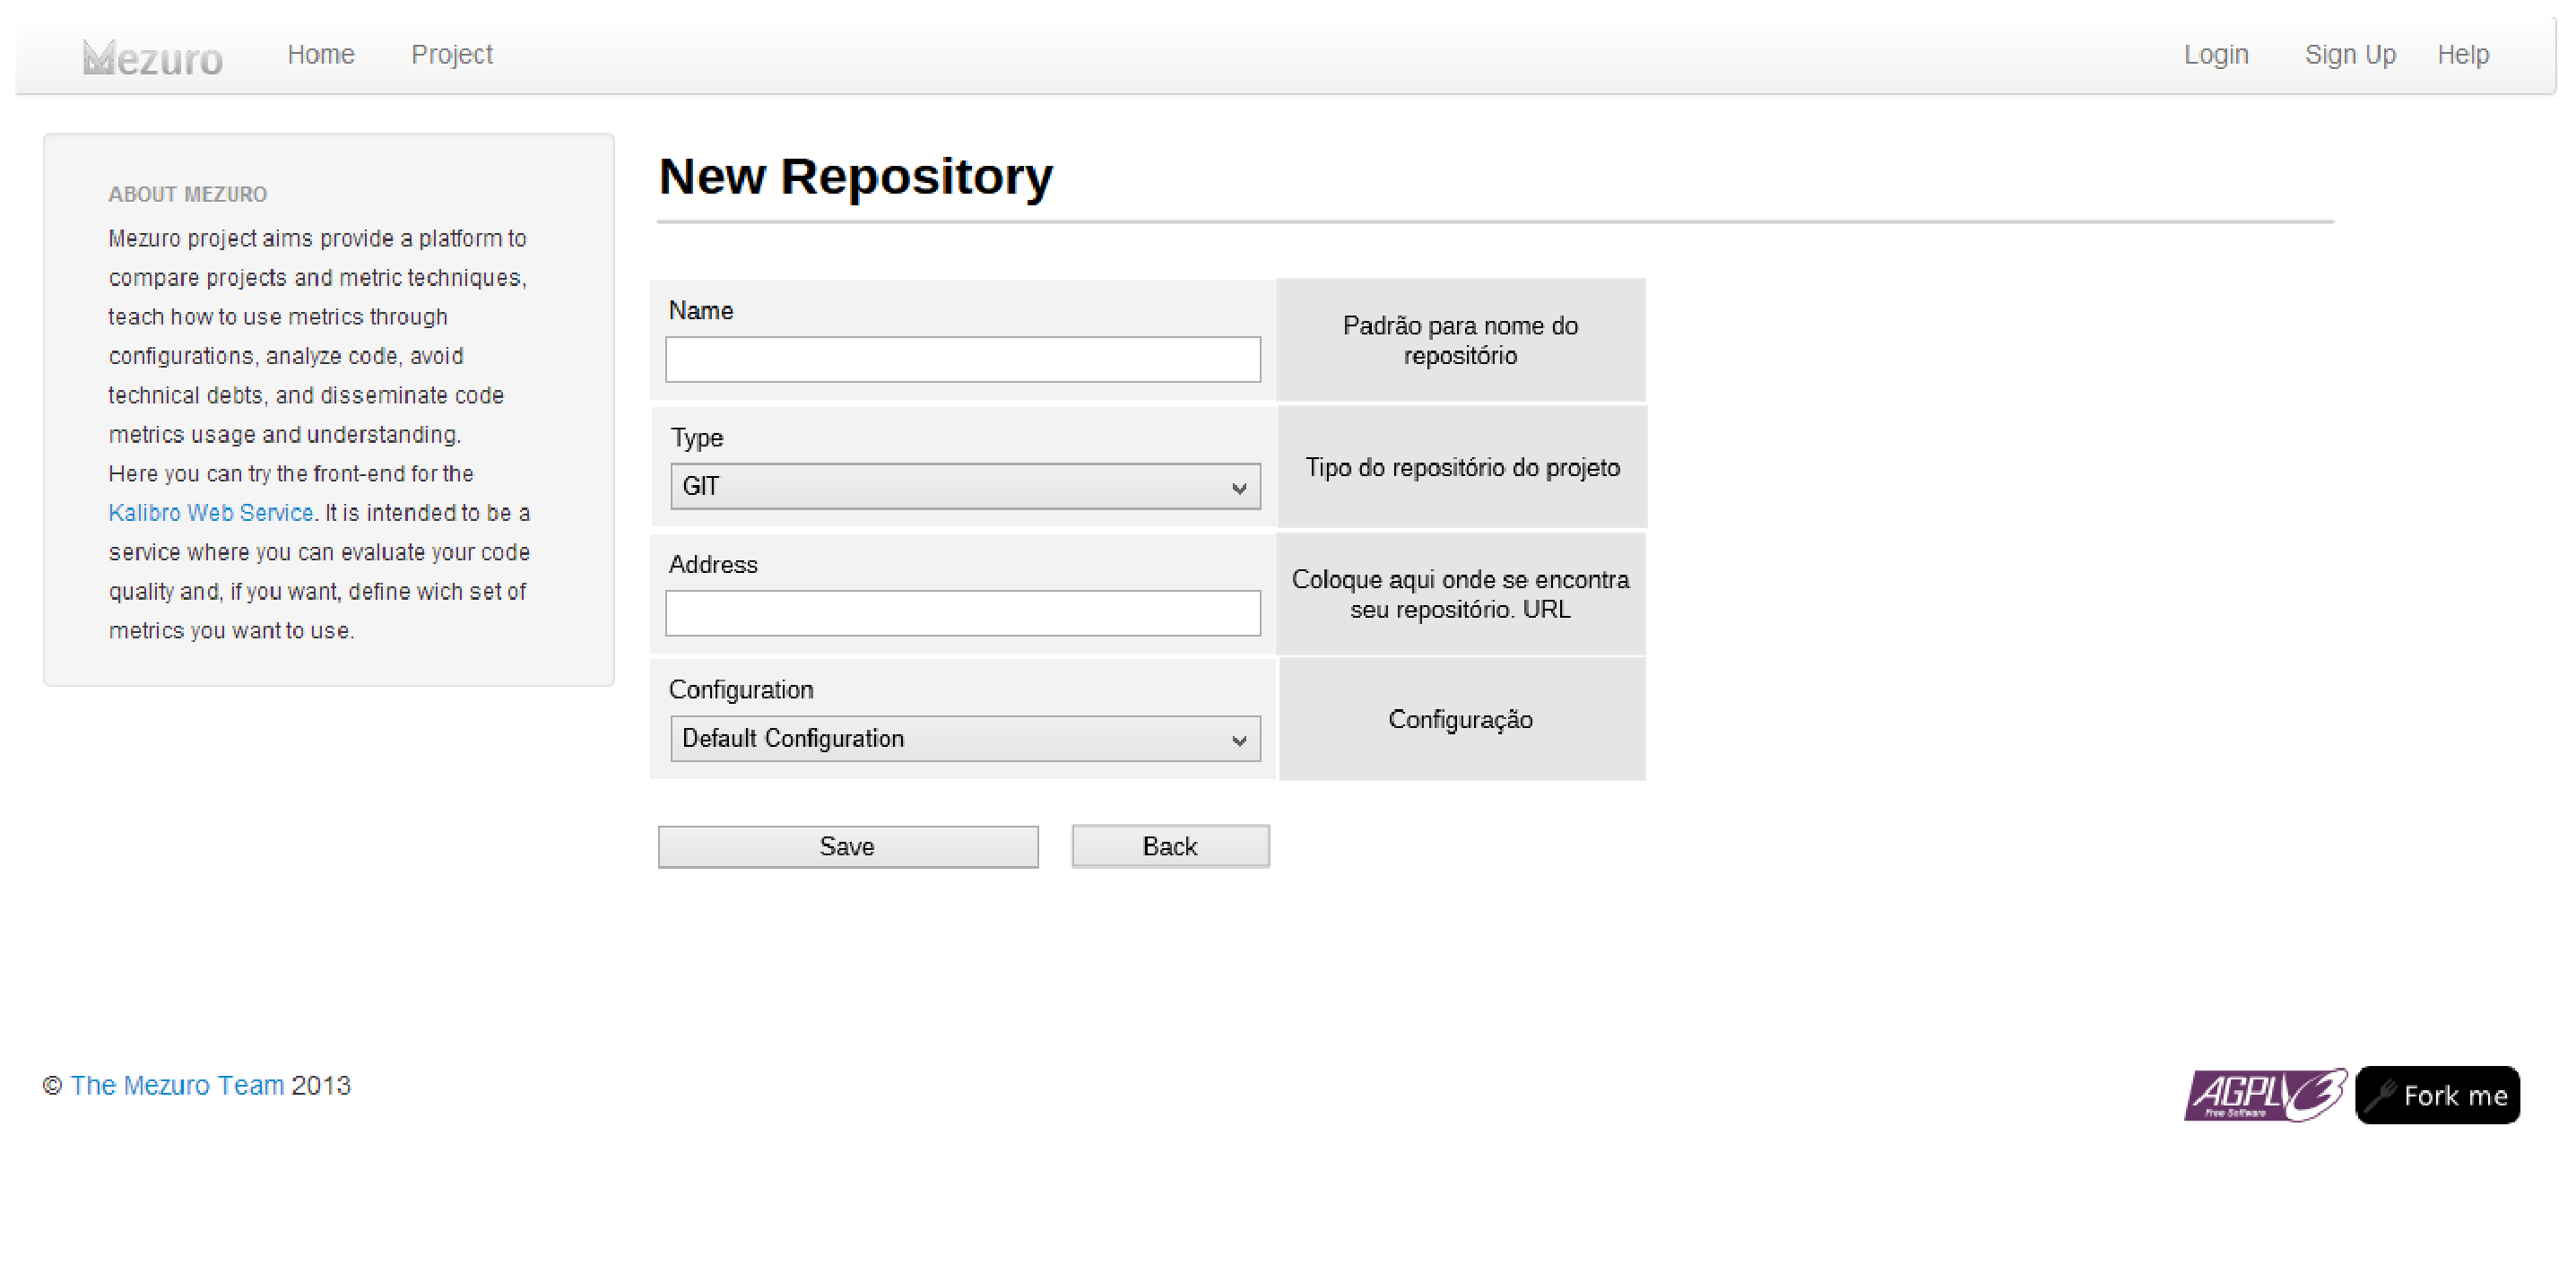
\includegraphics[width=1\textwidth]{figuras/NewRepository.eps}
    \caption{Protótipo de tela: New Repository}
    \label{fig:pNewRepository}
  \end{center}
\end{figure}

\begin{figure}[H]
  \begin{center}
    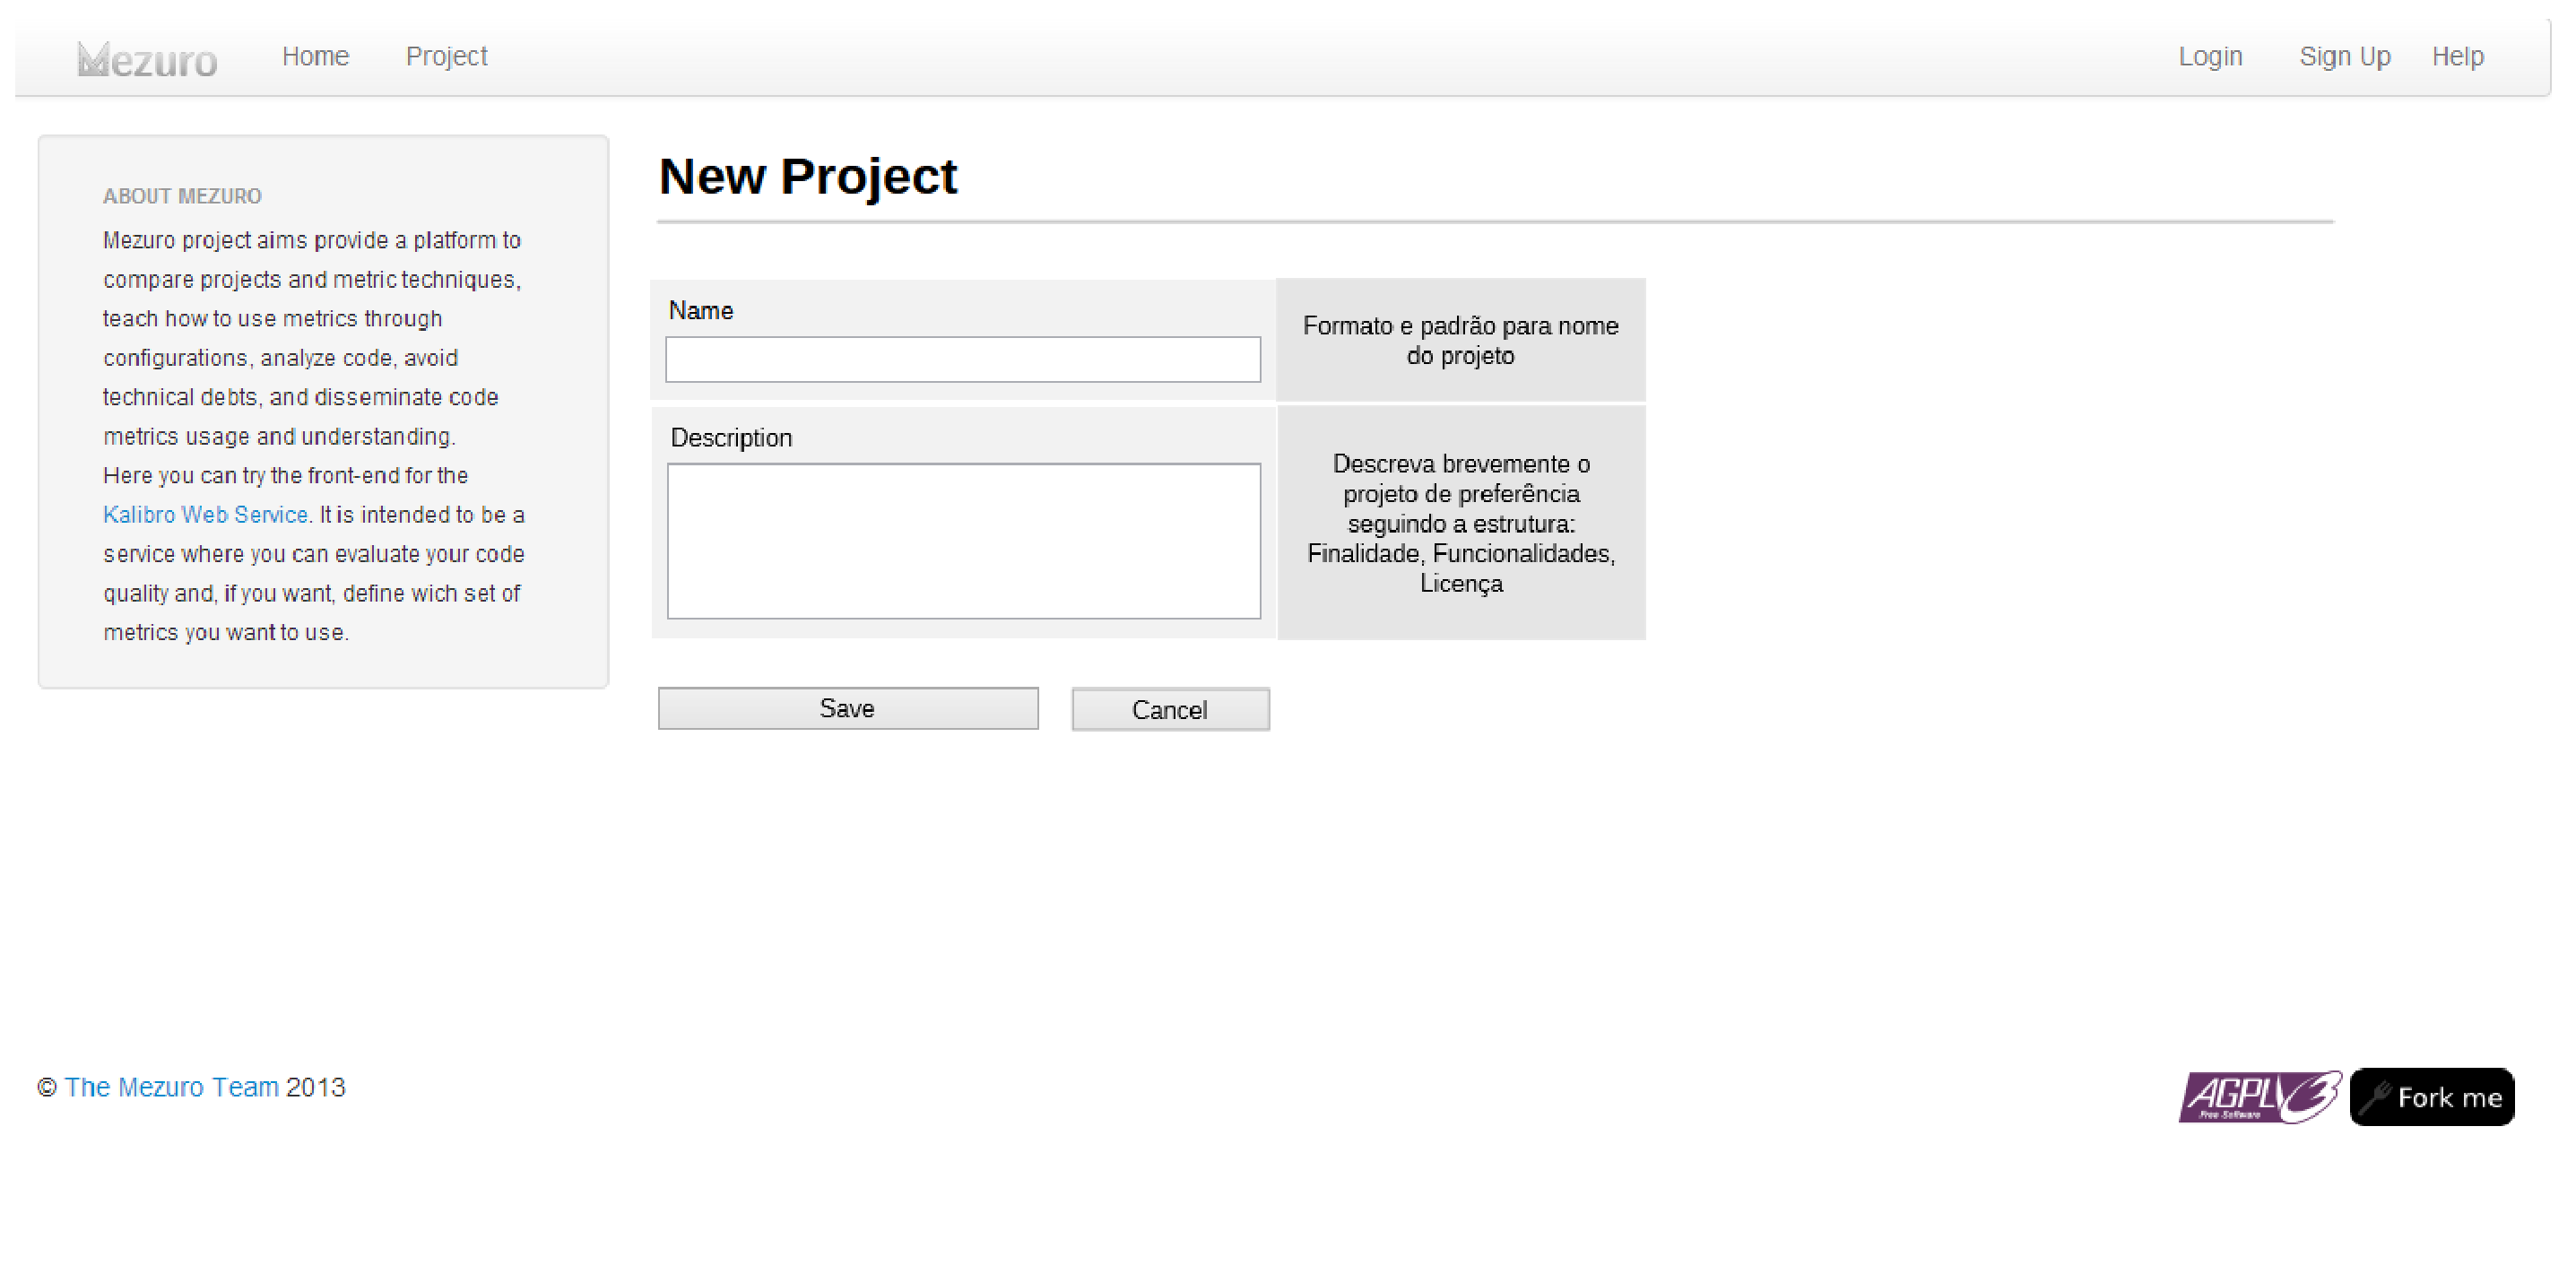
\includegraphics[width=1\textwidth]{figuras/NewProject.eps}
    \caption{Protótipo de tela: New Protótipo}
    \label{fig:pNewPrototipo}
  \end{center}
\end{figure}